\documentclass{article}\usepackage[]{graphicx}\usepackage[]{color}
%% maxwidth is the original width if it is less than linewidth
%% otherwise use linewidth (to make sure the graphics do not exceed the margin)
\makeatletter
\def\maxwidth{ %
  \ifdim\Gin@nat@width>\linewidth
    \linewidth
  \else
    \Gin@nat@width
  \fi
}
\makeatother

\definecolor{fgcolor}{rgb}{0.345, 0.345, 0.345}
\newcommand{\hlnum}[1]{\textcolor[rgb]{0.686,0.059,0.569}{#1}}%
\newcommand{\hlstr}[1]{\textcolor[rgb]{0.192,0.494,0.8}{#1}}%
\newcommand{\hlcom}[1]{\textcolor[rgb]{0.678,0.584,0.686}{\textit{#1}}}%
\newcommand{\hlopt}[1]{\textcolor[rgb]{0,0,0}{#1}}%
\newcommand{\hlstd}[1]{\textcolor[rgb]{0.345,0.345,0.345}{#1}}%
\newcommand{\hlkwa}[1]{\textcolor[rgb]{0.161,0.373,0.58}{\textbf{#1}}}%
\newcommand{\hlkwb}[1]{\textcolor[rgb]{0.69,0.353,0.396}{#1}}%
\newcommand{\hlkwc}[1]{\textcolor[rgb]{0.333,0.667,0.333}{#1}}%
\newcommand{\hlkwd}[1]{\textcolor[rgb]{0.737,0.353,0.396}{\textbf{#1}}}%
\let\hlipl\hlkwb

\usepackage{framed}
\makeatletter
\newenvironment{kframe}{%
 \def\at@end@of@kframe{}%
 \ifinner\ifhmode%
  \def\at@end@of@kframe{\end{minipage}}%
  \begin{minipage}{\columnwidth}%
 \fi\fi%
 \def\FrameCommand##1{\hskip\@totalleftmargin \hskip-\fboxsep
 \colorbox{shadecolor}{##1}\hskip-\fboxsep
     % There is no \\@totalrightmargin, so:
     \hskip-\linewidth \hskip-\@totalleftmargin \hskip\columnwidth}%
 \MakeFramed {\advance\hsize-\width
   \@totalleftmargin\z@ \linewidth\hsize
   \@setminipage}}%
 {\par\unskip\endMakeFramed%
 \at@end@of@kframe}
\makeatother

\definecolor{shadecolor}{rgb}{.97, .97, .97}
\definecolor{messagecolor}{rgb}{0, 0, 0}
\definecolor{warningcolor}{rgb}{1, 0, 1}
\definecolor{errorcolor}{rgb}{1, 0, 0}
\newenvironment{knitrout}{}{} % an empty environment to be redefined in TeX

\usepackage{alltt}

\usepackage{lineno}
\usepackage{enumitem}

\linenumbers

\title{Problem Set 3}
\author{Carrie Kathlyn Townley Flores, Filipe Recch, Kaylee Tuggle Matheny, \\ Klint Kanopka, Kritphong Mongkhonvanit \\ EDUC 252L}



\IfFileExists{upquote.sty}{\usepackage{upquote}}{}
\begin{document}
\maketitle

\section*{Shortish Answer}
\begin{enumerate}

\item Suppose that we have a test scaled with the Rasch model whose first 3 items have known difficulties -1, 0, and 1.5. An examinee with ability theta got the first item right, the second item right, and the third item wrong. Can you write the likelihood of observing this sequence of item responses as a function of theta?

$$ \frac{\epsilon^{\theta - d}}{1+\epsilon^{\theta - d}} $$ 

Item dif -1: $ \frac{\epsilon^{\theta + 1}}{1+\epsilon^{\theta + 1}} $ \\
Item dif 0: $ \frac{\epsilon^{\theta - 0}}{1+\epsilon^{\theta - 0}} $ \\
Item dif 1.5: $ \frac{\epsilon^{\theta + 1.5}}{1+\epsilon^{\theta + 1.5}} $ 

\item Can you plot this as a function of theta?

\begin{knitrout}
\definecolor{shadecolor}{rgb}{0.969, 0.969, 0.969}\color{fgcolor}\begin{kframe}
\begin{alltt}
\hlstd{th}\hlkwb{<-}\hlkwd{seq}\hlstd{(}\hlopt{-}\hlnum{3}\hlstd{,}\hlnum{3}\hlstd{,}\hlkwc{length.out}\hlstd{=}\hlnum{1000}\hlstd{)}
\hlstd{p}\hlkwb{<-}\hlkwa{function}\hlstd{(}\hlkwc{b}\hlstd{)} \hlkwd{exp}\hlstd{(th}\hlopt{-}\hlstd{b)}\hlopt{/}\hlstd{(}\hlnum{1}\hlopt{+}\hlkwd{exp}\hlstd{(th}\hlopt{-}\hlstd{b))}

\hlkwd{plot}\hlstd{(th,}\hlkwd{p}\hlstd{(}\hlopt{-}\hlnum{1}\hlstd{)}\hlopt{*}\hlkwd{p}\hlstd{(}\hlnum{0}\hlstd{)}\hlopt{*}\hlstd{(}\hlnum{1}\hlopt{-}\hlkwd{p}\hlstd{(}\hlopt{-}\hlnum{1.5}\hlstd{)),} \hlkwc{ylim} \hlstd{=} \hlkwd{c}\hlstd{(}\hlnum{0}\hlstd{,}\hlnum{.2}\hlstd{))} \hlcom{# question 4}
\end{alltt}
\end{kframe}
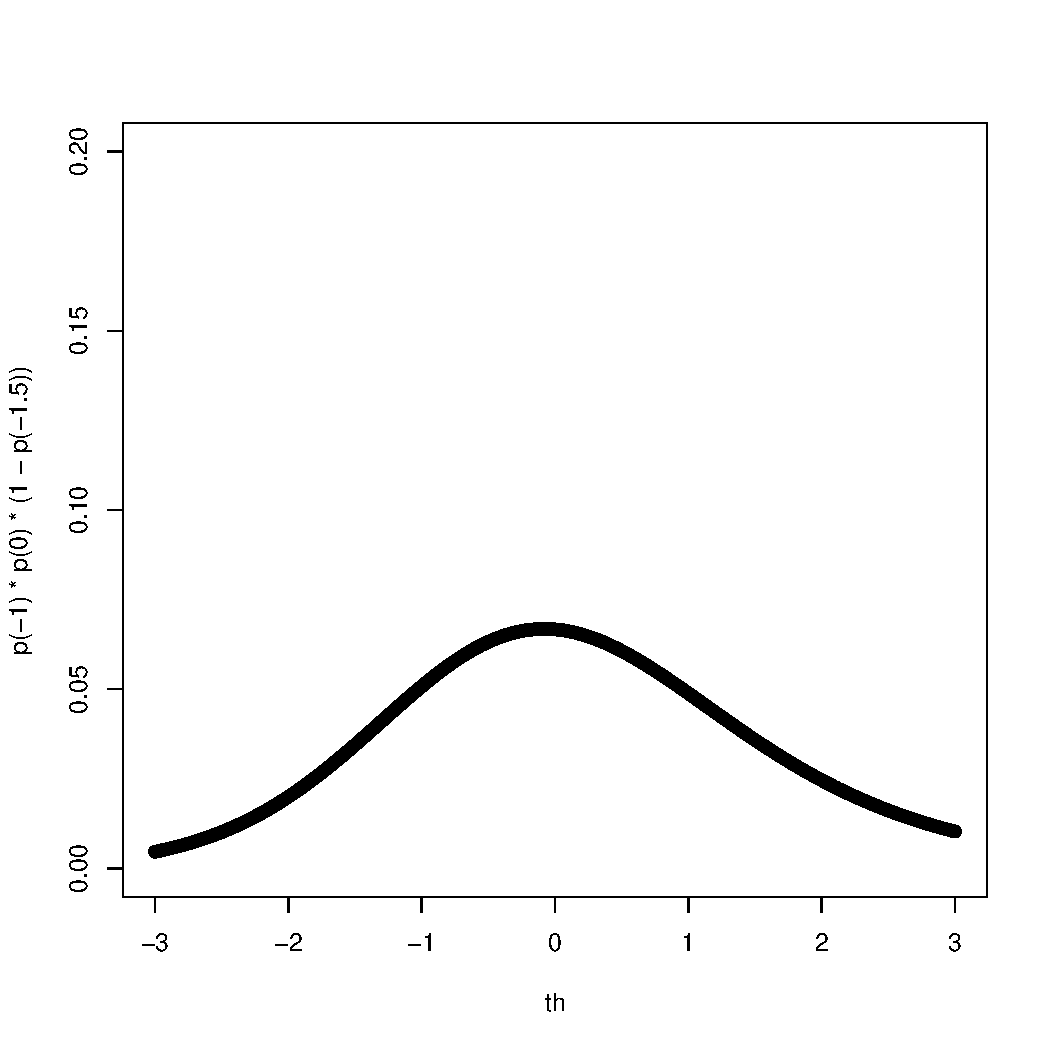
\includegraphics[width=\maxwidth]{figure/unnamed-chunk-2-1} 

\end{knitrout}

\item If theta=0.5, what is the likelihood of that response sequence?

\item If theta=0.5, what is the most likely response sequence given the known item difficulties? 

\item At what value of theta does a response sequence of 1-1-0 (that is: they got the first and second items right and the third item wrong) become more likely than a response sequence of 1-0-0?

\begin{knitrout}
\definecolor{shadecolor}{rgb}{0.969, 0.969, 0.969}\color{fgcolor}\begin{kframe}
\begin{alltt}
\hlkwd{plot}\hlstd{(th,}\hlkwd{p}\hlstd{(}\hlopt{-}\hlnum{1}\hlstd{)}\hlopt{*}\hlkwd{p}\hlstd{(}\hlnum{0}\hlstd{)}\hlopt{*}\hlstd{(}\hlnum{1}\hlopt{-}\hlkwd{p}\hlstd{(}\hlopt{-}\hlnum{1.5}\hlstd{)),} \hlkwc{ylim} \hlstd{=} \hlkwd{c}\hlstd{(}\hlnum{0}\hlstd{,}\hlnum{.2}\hlstd{))}
\hlkwd{lines}\hlstd{(th,}\hlkwd{p}\hlstd{(}\hlopt{-}\hlnum{1}\hlstd{)}\hlopt{*}\hlstd{(}\hlnum{1}\hlopt{-}\hlkwd{p}\hlstd{(}\hlnum{0}\hlstd{))}\hlopt{*}\hlstd{(}\hlnum{1}\hlopt{-}\hlkwd{p}\hlstd{(}\hlopt{-}\hlnum{1.5}\hlstd{)))} \hlcom{# question 5}
\end{alltt}
\end{kframe}
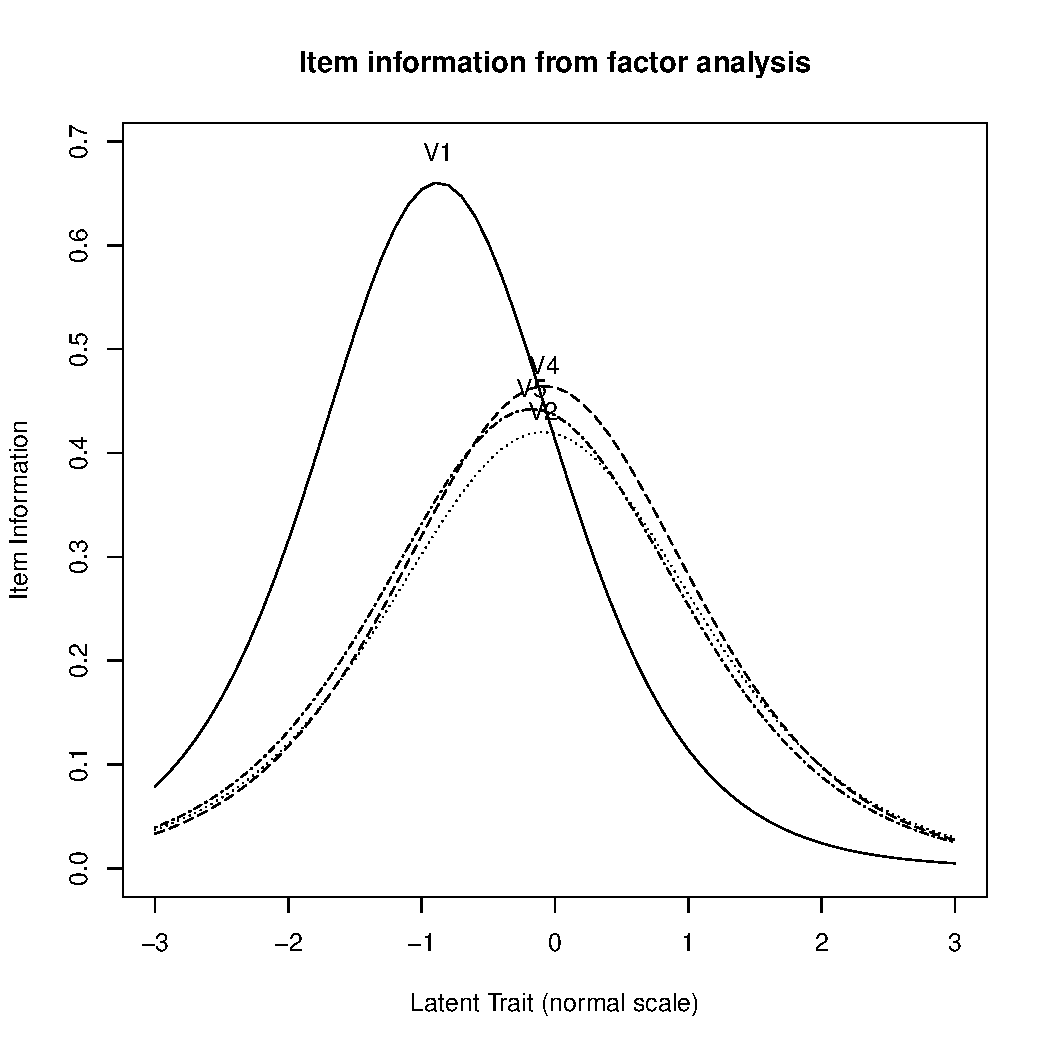
\includegraphics[width=\maxwidth]{figure/unnamed-chunk-3-1} 

\end{knitrout}


\item Returning to questions 1 and 2, can you plot the "test information" as a function of theta (see Eqn 2-6 in Lord). 

Sum of information function $ \sum IIF = TIF $

\item Where is the function in \#6 maximized? What do you think this implies? 

\item For an item response dataset of your choosing, consider the relationship between theta and the SE across the three IRT models for dichotomous items. How much of a difference does the choice of model have on the size of the error estimate?

\end{enumerate}

\end{document}
